A nível de preparação de dados pouco foi feito, no entanto é importante denotar os seguintes aspectos chaves, que foram cruciais na nossa investigação.

\begin{itemize}
    \item A atributo \texttt{gameID} é completamente irrelevante pois é uma chave única associada a cada jogo, sem nenhum tipo de relevància física, por isso esse atributo foi removido.
    \item Os atributos \texttt{blueWins} e \texttt{redWins} são ambos binários e disjuntos, o que significa que a soma será sempre 1, pois numa dada partida apenas uma equipa pode ganhar. Como tal, consideramos apenas o atributo \texttt{blueWins}, tornando o problema num de prever a vitória ou derrota desta mesma equipa.
    \item De igual forma, os atributos \texttt{blueFirstBlood} e \texttt{redFirstBlood} seguem a mesma condição, pelo que só vale a pena ponderar um destes atributos.
    \item Nos restantes atributos, considerar tanto os atributos da equipa azul e vermelha não faz sentido. Na verdade, estamos interessados em perceber qual a diferença entre os resultados obtidos pela equipa azul num dado atributo e aqueles obtidos pela equipa vermelha. Assim sendo, os restantes atributos, 36, foram reduzidos a 18 por via de \textit{feature engineering}, sendo que no final os atributos em si passam a representar a diferença entre as 2 equipas.
\end{itemize}

Com isto em mente, podemos agora analisar as correlações existentes de forma mais compreensível.

\begin{figure}[H]
    \centering
    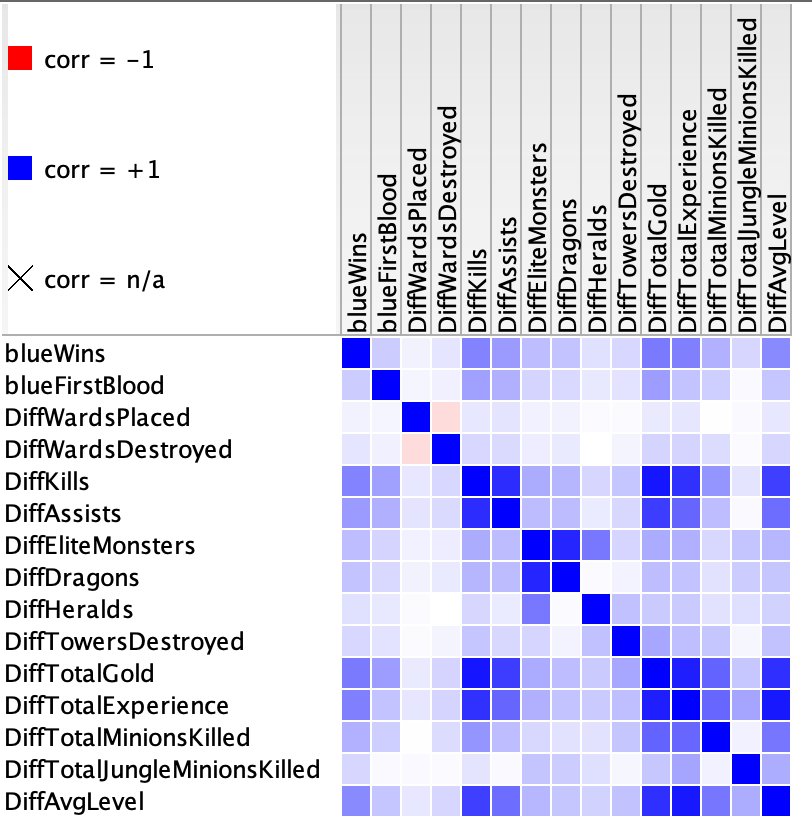
\includegraphics[width=0.5\linewidth]{Figures/RankCorrelation.png}
    \caption{Correlação entre features após processamento.}
    \label{fig:corr1}
\end{figure}

Pela figura \ref{fig:corr1} conseguimos detetar algumas correlações menos óbvios do que obtidas anteriormente. Por exemplo, podemos observar que a diferença em kills está fortemente correlacionada positivamente à diferença em ouro entre as duas equipas.

\begin{figure}[H]
    \centering
    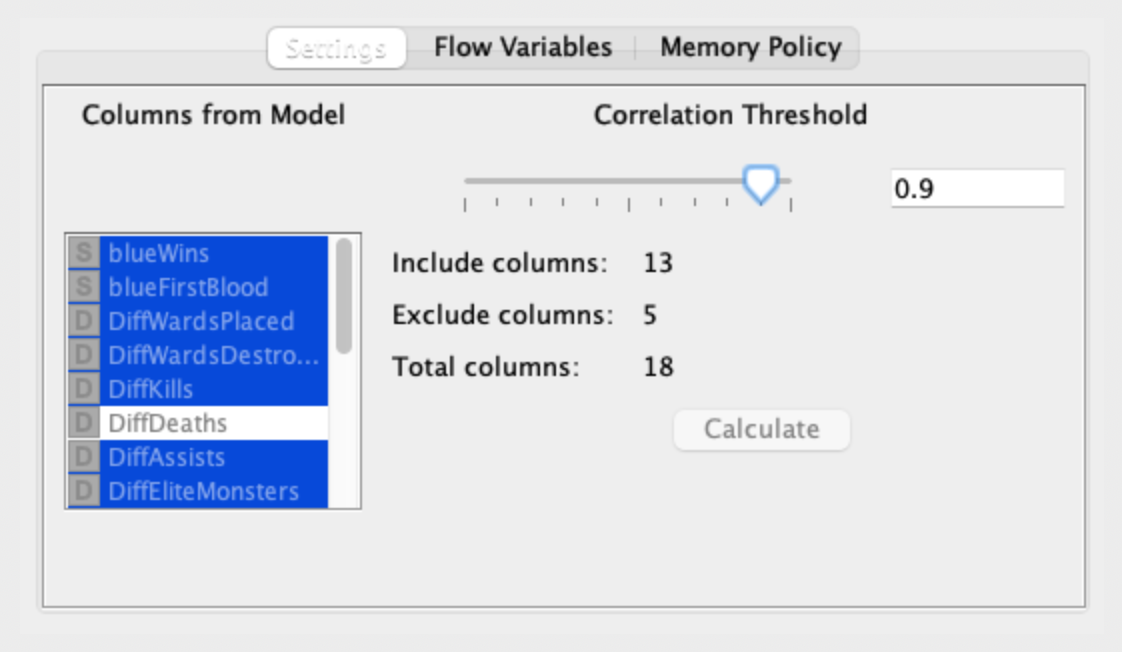
\includegraphics[width=0.5\linewidth]{Figures/Screenshot_2020-11-25_at_22.10.32.png}
    \caption{Seleção automática de features correlacionadas.}
    \label{fig:corr2}
\end{figure}


Como é desnecessário considerar atributos fortemente correlacionados entre si, utilizamos um correlation filter com as configurações da figura \ref{fig:corr2}.